% 1977 年宁夏卷第 15 题：平顶大正六边形 ABCDEF，各边上的分点 A'、B'、C'、D'、E'、F'
% 连成内接小正六边形；AA' 段标 m，A'B 段标 n（按源卷第 4 页布局）
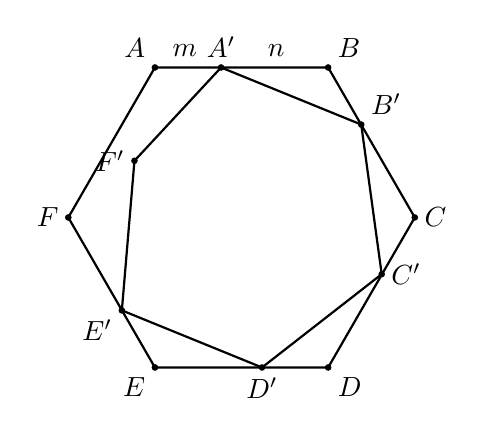
\begin{tikzpicture}[scale=1.0]
  \coordinate (A) at (-1.1,1.905);
  \coordinate (B) at (1.1,1.905);
  \coordinate (C) at (2.2,0);
  \coordinate (D) at (1.1,-1.905);
  \coordinate (E) at (-1.1,-1.905);
  \coordinate (F) at (-2.2,0);
  \coordinate (Ap) at (-0.26,1.905);
  \coordinate (Bp) at (1.52,1.18);
  \coordinate (Cp) at (1.78,-0.72);
  \coordinate (Dp) at (0.26,-1.905);
  \coordinate (Ep) at (-1.52,-1.18);
  \coordinate (Fp) at (-1.36,0.72);
  \draw[thick] (A)--(B)--(C)--(D)--(E)--(F)--cycle;
  \draw[thick] (Ap)--(Bp)--(Cp)--(Dp)--(Ep)--(Fp)--cycle;
  \fill (A) circle (1.2pt) node[above left] {$A$};
  \fill (B) circle (1.2pt) node[above right] {$B$};
  \fill (C) circle (1.2pt) node[right] {$C$};
  \fill (D) circle (1.2pt) node[below right] {$D$};
  \fill (E) circle (1.2pt) node[below left] {$E$};
  \fill (F) circle (1.2pt) node[left] {$F$};
  \fill (Ap) circle (1.2pt) node[above] {$A'$};
  \fill (Bp) circle (1.2pt) node[above right] {$B'$};
  \fill (Cp) circle (1.2pt) node[right] {$C'$};
  \fill (Dp) circle (1.2pt) node[below] {$D'$};
  \fill (Ep) circle (1.2pt) node[below left] {$E'$};
  \fill (Fp) circle (1.2pt) node[left] {$F'$};
  \node at (-0.72,2.12) {$m$};
  \node at (0.44,2.12) {$n$};
\end{tikzpicture}
